\chapter{Theoretical Background}
\label{chap:background}

This chapter introduces the key concepts and methods used in this thesis. The focus is on techniques relevant to sequential decision-making and adaptive experimentation in email campaign optimization. Since these concepts are well established in the literature, only the essential ideas required to understand the methodology are presented.

\section{A/B Testing}

A/B testing is a statistical method used to compare two or more variants of a design by randomly assigning users to different groups and measuring a target metric such as click-through rate or conversion rate~\cite{kohavi2009controlled}. In email marketing, it is commonly applied to evaluate variations in subject lines, layouts, or call-to-action elements. Despite its widespread use, A/B testing has well-documented limitations: it requires large traffic volumes to reach statistical significance, does not adapt during the experiment, and cannot personalize decisions to individual users~\cite{deng2013improving}.

\begin{figure}[htbp]
    \centering
    \begin{tikzpicture}[
        node distance=0.5cm and 0.9cm,
        box/.style={rectangle, draw, rounded corners=3pt, fill=gray!10,
                    text width=2.6cm, align=center, minimum height=0.9cm, font=\small},
        arr/.style={->, thick, >=stealth}
    ]
        \node[box] (traffic) {Recipients \\ (100\,\%)};
        \node[box, above right=of traffic] (va) {Variant $A$ \\ (50\,\%)};
        \node[box, below right=of traffic] (vb) {Variant $B$ \\ (50\,\%)};
        \node[box, below right=of va] (test) {Significance test};
        \node[box, right=of test] (winner) {Winner applied \\ to all recipients};
        \draw[arr] (traffic) -- (va);
        \draw[arr] (traffic) -- (vb);
        \draw[arr] (va) -- (test);
        \draw[arr] (vb) -- (test);
        \draw[arr] (test) -- (winner);
    \end{tikzpicture}
    \caption{Classical A/B test: traffic is split evenly for the full duration of the
    experiment; only after the test ends is the winning variant applied.}
    \label{fig:ab_split}
\end{figure}

\section{Bayesian Inference}

Bayesian inference provides a probabilistic framework for updating beliefs based on observed data~\cite{scott2010modern}. Rather than treating campaign performance as a fixed unknown quantity estimated from a single batch, Bayesian methods maintain a probability distribution over possible performance values and update it continuously as new observations arrive. This makes Bayesian inference particularly suitable for online settings where decisions must be made before all data is collected.

Bayesian inference is based on Bayes' theorem:
\begin{equation}
    \underbrace{P(\theta \mid D)}_{\text{posterior}}
    \propto
    \underbrace{P(D \mid \theta)}_{\text{likelihood}} \cdot
    \underbrace{P(\theta)}_{\text{prior}},
\end{equation}
where the prior encodes the belief about the unknown quantity $\theta$ before observing data $D$, and the posterior is the updated belief afterwards. In this thesis, $\theta$ is a click probability, modeled with a $\mathrm{Beta}(\alpha,\beta)$ distribution whose parameters count observed successes and failures; a belief update therefore reduces to counting. For example, starting from the uninformative prior $\mathrm{Beta}(1,1)$ and observing 3 clicks in 10 sends yields the posterior $\mathrm{Beta}(4,8)$ with mean $4/12 \approx 0.33$ (Figure~\ref{fig:beta_update}).

\begin{figure}[htbp]
    \centering
    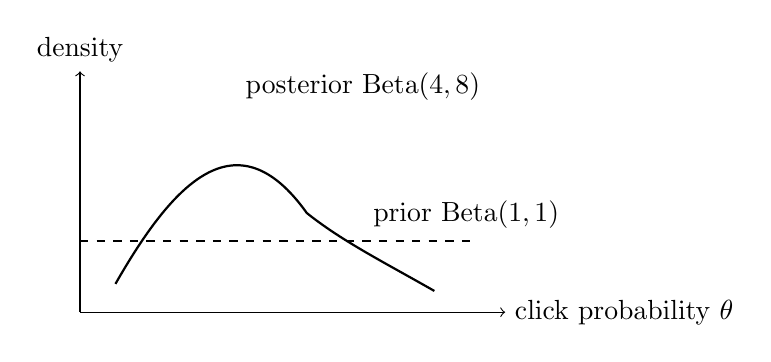
\begin{tikzpicture}[scale=0.9]
        \draw[->] (0,0) -- (6,0) node[right] {click probability $\theta$};
        \draw[->] (0,0) -- (0,3.4) node[above] {density};
        \draw[thick, dashed] (0,1) -- (5.5,1);
        \draw[thick] (0.5,0.4) .. controls (1.3,1.8) and (2.2,2.8) .. (3.2,1.4)
                    .. controls (3.7,1.0) and (4.3,0.7) .. (5.0,0.3);
        \node[anchor=south west] at (4.0,1.05) {prior $\mathrm{Beta}(1,1)$};
        \node[anchor=south west] at (2.2,2.85) {posterior $\mathrm{Beta}(4,8)$};
    \end{tikzpicture}
    \caption{Belief update in the worked example: observing 3 clicks out of 10 sends
    turns a flat prior into a posterior concentrated around $\theta \approx 0.33$.}
    \label{fig:beta_update}
\end{figure}

\section{Multi-Armed Bandits}
\label{sec:bg_mab}

The multi-armed bandit problem models sequential decision-making under uncertainty~\cite{auer2002finite}. It is defined by a set of $K$ \emph{arms} (candidate actions, e.g., email variants) $\mathcal{A} = \{1, \dots, K\}$, each with an unknown expected reward $\mu_a$; at each round $t$, the learner selects one arm $a_t$ and observes only the reward of that arm. The goal is to maximize cumulative reward over time by balancing the need to test uncertain arms (exploration) against the need to favor arms already known to perform well (exploitation). Bandit algorithms address this trade-off algorithmically, making them a natural replacement for A/B testing in dynamic optimization settings.

Bandit algorithms are compared by their \emph{regret}, the cumulative reward lost relative to always playing the best arm $a^{*} = \arg\max_a \mu_a$:
\begin{equation}
    R(T) \;=\; T \mu_{a^{*}} \;-\; \mathbb{E}\!\left[\sum_{t=1}^{T} \mu_{a_t}\right];
    \label{eq:regret}
\end{equation}
lower regret means faster convergence to the optimal arm.

\section{Thompson Sampling}

Thompson Sampling is a Bayesian approach to the multi-armed bandit problem~\cite{chapelle2011empirical}, shown in Algorithm~\ref{alg:thompson}. At each decision point, it samples a reward estimate from the current posterior distribution of each arm and selects the arm with the highest sampled value. This naturally balances exploration and exploitation: arms with high uncertainty are explored more often because their samples are more variable, while arms with well-established high performance are exploited more consistently. Empirically, Thompson Sampling converges faster than alternatives such as epsilon-greedy or UCB strategies~\cite{chapelle2011empirical}.

\begin{algorithm}[htbp]
\caption{Thompson Sampling with Beta--Bernoulli posteriors}
\label{alg:thompson}
\begin{algorithmic}[1]
\State Initialize $\alpha_a \gets 1$, $\beta_a \gets 1$ for every arm $a \in \{1,\dots,K\}$
\For{round $t = 1, 2, \dots, T$}
    \State Sample $\tilde{\theta}_a \sim \mathrm{Beta}(\alpha_a, \beta_a)$ for each arm $a$
    \State Play arm $a_t \gets \arg\max_a \tilde{\theta}_a$ \Comment{send this email variant}
    \State Observe reward $r_t \in \{0, 1\}$ \Comment{click or no click}
    \State $\alpha_{a_t} \gets \alpha_{a_t} + r_t$; \quad $\beta_{a_t} \gets \beta_{a_t} + (1 - r_t)$
\EndFor
\end{algorithmic}
\end{algorithm}

\section{Contextual Bandits}

Contextual bandits extend the multi-armed bandit framework by conditioning decisions on observable features of the current user or environment, referred to as the context~\cite{li2010contextual}. In email marketing, context may include device type, geographic region, time of day, or past engagement behavior. This allows the algorithm to learn different optimal actions for different user profiles, enabling personalization rather than applying a single winning variant to all recipients.

\section{Reinforcement Learning}
\label{sec:bg_rl}

Reinforcement Learning (RL) provides a general framework for sequential decision-making in which an agent learns to maximize long-term cumulative reward through repeated interaction with an environment~\cite{sutton2018reinforcement}, modeled as a Markov Decision Process $\mathcal{M} = (\mathcal{S}, \mathcal{A}, P, R, \gamma)$ with states $\mathcal{S}$, actions $\mathcal{A}$, transition probabilities $P$, rewards $R$, and discount factor $\gamma$ (Figure~\ref{fig:rl_loop}). A bandit is the special case of an MDP with a single state, in which every decision is independent and only the immediate reward matters. Full RL is required when actions change the state and thereby affect future rewards --- as in email drip campaigns, where the response to an earlier message changes the recipient's state and should influence the design of later ones.

\begin{figure}[htbp]
    \centering
    \begin{tikzpicture}[
        box/.style={rectangle, draw, rounded corners=3pt, fill=gray!10,
                    text width=3.2cm, align=center, minimum height=1.0cm, font=\small},
        arr/.style={->, thick, >=stealth}
    ]
        \node[box] (agent) {Agent \\ (policy $\pi$)};
        \node[box, right=3.6cm of agent] (env) {Environment \\ (recipient journey)};
        \draw[arr] (agent.north east) to[bend left=18]
            node[above, font=\small]{action $a_t$} (env.north west);
        \draw[arr] (env.south west) to[bend left=18]
            node[below, font=\small]{reward $r_t$, next state $s_{t+1}$} (agent.south east);
    \end{tikzpicture}
    \caption{Reinforcement learning loop. A bandit follows the same loop but without a
    state: each round is independent.}
    \label{fig:rl_loop}
\end{figure}

\section{Evaluation Metrics}

Campaign performance is measured using standard email marketing metrics. Let $n_{\mathrm{del}}$ be the number of delivered emails, $n_{\mathrm{open}}$ the number opened, $n_{\mathrm{click}}$ the number of opened emails in which a link was clicked, and $n_{\mathrm{conv}}$ the number of recipients completing the target action after clicking:
\begin{align}
    \text{open rate} &= \frac{n_{\mathrm{open}}}{n_{\mathrm{del}}}, &
    \text{click-through rate (CTR)} &= \frac{n_{\mathrm{click}}}{n_{\mathrm{open}}}, &
    \text{conversion rate} &= \frac{n_{\mathrm{conv}}}{n_{\mathrm{click}}}.
\end{align}
In addition, the adaptive methods are compared on convergence speed using the cumulative regret of Equation~\eqref{eq:regret}.

\section{Comparison of the Methods}
\label{sec:bg_comparison}

Table~\ref{tab:method_comparison} summarizes the four methods along the dimensions relevant to this thesis.

\begin{table}[htbp]
    \centering
    \caption{Comparison of the four optimization methods evaluated in this thesis.}
    \label{tab:method_comparison}
    \small
    \begin{tabular}{lcccc}
        \toprule
        Property & A/B testing & Thompson Sampling & Contextual bandit & RL \\
        \midrule
        Adapts during experiment      & no  & yes & yes & yes \\
        Uses user context             & no  & no  & yes & yes \\
        Personalized decisions        & no  & no  & yes & yes \\
        Models multi-step sequences   & no  & no  & no  & yes \\
        Data requirement              & low & low & medium & high \\
        Implementation complexity     & low & low & medium & high \\
        \bottomrule
    \end{tabular}
\end{table}
